\documentclass{article}
\usepackage[utf8]{inputenc}
\usepackage{amsmath}
\usepackage{graphicx} %for images
\usepackage[utf8]{inputenc} %for ToC
\usepackage{lscape}%for landscape layout
\usepackage{rotating}%to rotate figs
\usepackage{geometry}%to change margins
\usepackage{hyperref} %for links
\hypersetup{
linktoc=all,  
    colorlinks,
    citecolor=black,
    filecolor=black,
    linkcolor=black,
    urlcolor=black
}

%for bibliography"
%with biblatex
%\usepackage[style=authoryear]{biblatex}
%\addbibresource{references.bib}
% or with natbib
\usepackage{natbib} 
\usepackage{har2nat}
%\bibliography{references.bib}

\renewenvironment{abstract}
 {\normalsize
  \begin{center}
  \bfseries \large \abstractname \vspace{-.5em}\vspace{0pt}
  \end{center}
  \list{}{
    \setlength{\leftmargin}{.5cm}%
    \setlength{\rightmargin}{\leftmargin}%
  }%
  \item\relax}
 {\endlist}

\begin{document}
\pagenumbering{roman}
%\begin{titlepage}
    \begin{center}
          

        \Huge
        \textbf{Understanding how pharmaceutical pollutants move through river catchments}
     
        \vspace{0.5cm}
        
        \normalsize
        \textbf{*Julia Costescu$^1^,^2$, Louise Bracken$^1^,^2$,
          Laura Turnbull-Lloyd$^1^,^2$,
            and Damian Crilly$^2^,^3$}
        
        
        
    
        \normalsizie
        Geography Department$^1$\\
        i-CONN Network$^2$\\
        Environment Agency$^3$\\

            
    \end{center}


%\clearpage
%\title{Progression paper}
%\title{Understanding how pharmaceutical pollutants move through river catchments}
%\author{Julia Costescu}
%\date{February 2021}

%\end{titlepage}

\vspace{0.5cm}
\begin{abstract} \addcontentsline{toc}{section}{Abstract}
Due to the risks it poses to non-target organisms and public health, the near ubiquitous presence of pharmaceutical compounds in environmental waters represents an emerging cause for concern, particularly in the context of increasing usage of human and veterinary pharmaceuticals on a global scale. Despite expanding research in the field, gaps remain in our understanding of how pharmaceuticals enter and travel through river catchments, and a more holistic approach is needed in order to develop effective management strategies that conform to the catchment-based approach. In this paper, we aim to add to this understanding by combining the analysis of both existing pharmaceutical data in the North East region of the UK and field data collected in a target catchment. This paper details the framework that underpins the proposed system-based approach, bringing together the source-pathway-receptor model, integrated catchment management and connectivity science. Subsequently, exploratory analyses and a provisional sampling strategy are used to characterize the spatiotemporal variability of pharmaceutical concentrations in the catchment. The results of this exploration will then inform the development of a network model that is expected to provide tools to aid decision-making on a catchment-level.
\end{abstract}
\clearpage
\vspace{0.5cm}
\tableofcontents



\clearpage

\pagenumbering{arabic}
\section{Introduction}

\clearpage
\section{Methods}

\clearpage
\section{Results}
\begin{figure}[!hb]
    \centering
    \includegraphics[height=8cm]{fig}
    \caption{Seasonality of concentrations (obtained by LC-MS) at the Nether Poppleton (Skelton) sampling site (Ouse catchment) for (a) Gabapentin, (b) Diclofenac, (c) Lidocaine. For each: (top) concentrations plotted by date across the years 2015-2020 with trend line and confidence interval; (bottom) seasonal trendlines grouped by year.}
    \label{fig_ouse_site_seasonality}
\end{figure}

\begin{figure}[!hb]
    \centering
    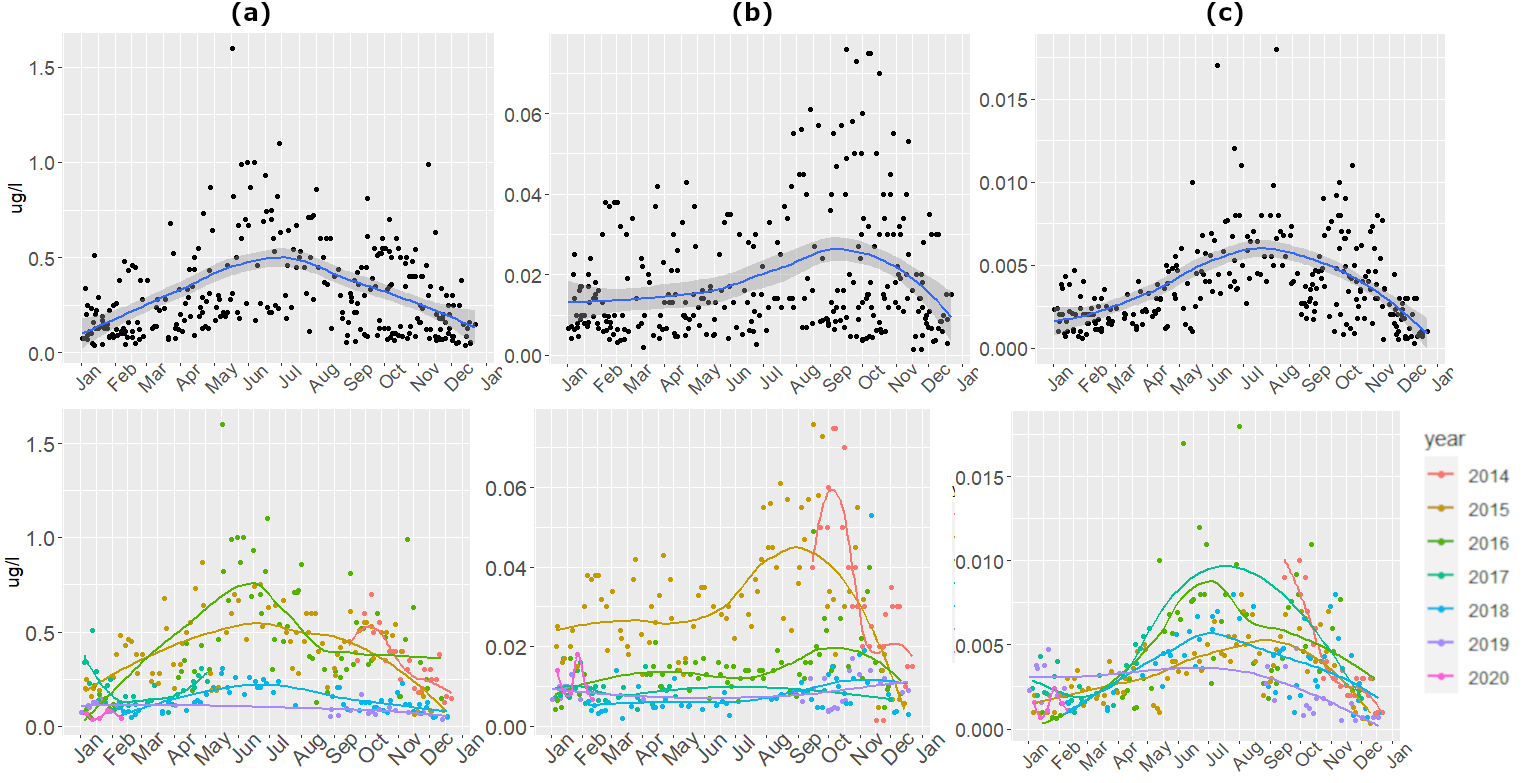
\includegraphics[height=8cm]{fig_seasonality.png}
    \caption{Seasonality of concentrations (obtained by LC-MS) at the Nether Poppleton (Skelton) sampling site (Ouse catchment) for (a) Gabapentin, (b) Diclofenac, (c) Lidocaine. For each: (top) concentrations plotted by date across the years 2015-2020 with trend line and confidence interval; (bottom) seasonal trendlines grouped by year.}
    \label{fig_ouse_site_seasonality}
\end{figure}



\clearpage
\section{Discussion}

%\printbibliography{references.bib} %with biblatex
\clearpage
%\bibliographystyle{agsm}

\addcontentsline{toc}{section}{References}
\bibliographystyle{elsarticle-harv}
\bibliography{references}


\end{document}
